% Created 2013-11-05 Tue 17:40
\documentclass[11pt]{article}
\usepackage[utf8]{inputenc}
\usepackage[T1]{fontenc}
\usepackage{graphicx}
\usepackage{longtable}
\usepackage{float}
\usepackage{wrapfig}
\usepackage{soul}
\usepackage{amssymb}
\usepackage{hyperref}
\usepackage{svn}
\usepackage[T1]{fontenc}
\usepackage{mathpazo}
\usepackage[margin=1.3in]{geometry}
\linespread{1.05}
\usepackage[scaled]{helvet}
\usepackage{courier}
\usepackage{varioref}
\usepackage[usenames,dvipsnames]{color}
\usepackage{hyperref}
\hypersetup{colorlinks=true,linkcolor=blue,urlcolor=RawSienna}
\floatplacement{figure}{H}
\floatplacement{table}{H}
\newcommand{\hilight}[1]{\colorbox{yellow}{#1}}

\title{Design Specifications for ``Hosting of Virtual-labs using the one-lab-per-vm model''}
\author{Suraj Samal}
\date{05 November 2013}

\begin{document}

\maketitle

\setcounter{tocdepth}{3}
\tableofcontents
\vspace*{1cm}
\listoftables
\listoffigures

\section{Introduction}
\label{sec-1}


   The document discusses the design of the overall architecture of
   the hosting of virtual-labs using the one-lab-per-vm model. This is
   as per the requirements specified in ``Minutes of the 2013-07-25 Thu
   Expert Committee meeting evaluating VLEAD’s progress in virtual lab
   integration'' document at \textbf{Section-4}, \textbf{Item-3}

   VLEAD (Virtual Labs Engineering and Architecture Division) team was
   setup in June 2012 as a central engineering team for integrating
   all the virtual-labs (around 180 in number) across all disciplines
   and institutes onto a common data-center (currently located at IIIT
   Hyderabad). Currently(as of 2013-11-01) around 100 labs are
   version-controlled and around 50 hosted out of IIIT data-centre.

\section{Document Revision}
\label{sec-2}


\begin{description}
\item [Current Revision] 0.1
\item [Revision Date] 2013-11-04
\end{description}
\section{Basic Architecture}
\label{sec-3}

\subsection{Overview}
\label{sec-3.1}

   Below is an overview of the overall system describing all the
   actors, entities and their interfaces:
   \hyperref[[[file:overview.jpg]{file:overview.jpg} ]]
\subsection{Actors}
\label{sec-3.2}

\subsubsection{Lab Developer}
\label{sec-3.2.1}

   An person who has agreed to use the services of VLEAD as per the
   \textbf{terms of association} and follows certain standard processes to
   maintain his/her lab during its development life-cycle. In
   specific, the roles are as follows:
\begin{itemize}
\item Checkin the lab contents (sources,dependencies, scripts and other files) into a lab-depository.
\item Keep updating the lab-depository with newer revisons of lab contents.
\item Instantiate a test lab-instance for testing and debugging issues.
\item Instantiate a live lab-instance.
\item View live lab-instance statistics.
\end{itemize}
\subsubsection{Lab Administrator}
\label{sec-3.2.2}

   An actor who is responsible for administering all the hosted
   labs. In specific, the roles are as follows:
\begin{itemize}
\item Allocate a unique labid and a depository(collection of
       repositories) to a lab
\item Allocation of resources(physical machines,ip address pools,
       vmid pools) to the labmanager and vmmanager
\end{itemize}
\subsubsection{Lab User}
\label{sec-3.2.3}

   These are end-users who use the virtual-labs and its experiments
\subsection{Entities}
\label{sec-3.3}

\subsubsection{LabDepository}
\label{sec-3.3.1}


     All labs are allocated a unique-id and a lab-depository by the
     labs administrator. A lab-depository represents a collection of
     various repositories associated with a lab.

\begin{description}
\item [lab-depository -] An \textbf{Object} describing the property of all
                    repositories of a particular lab

\begin{description}
\item [labid -] Unique identifier of the lab
\item [labinfo -] \textbf{Object} describing basic properties of a lab

\begin{description}
\item [labinst -] One of the defined \textbf{enumerations} ( IITB, IITK, IIITH ,,,)
\item [labdisc -] One of the defined \textbf{enumerations} ( chemical, mechanical \ldots{}..)
\item [labos -] \textbf{Object} describing a particular operating-system version

\begin{description}
\item [osname -] Name of the operating system
\item [osversion -] Specific version of the operating system
\end{description}

\end{description}

\item [repos -] Collection of repositories

\begin{description}
\item [metadata -]  A structured \textbf{object} representation of
                           depository contents describing the number
                           of repos present, actual repos present,
                           their type . This repository is regenerated
                           everytime the lab-developer makes a commit
                           to other repositories.

\begin{itemize}
\item [numrepos -] Total number of repositories present
\item [repoid1 -] Identification of each repositories
\item [repoid1 -]repoid2 -
\item [repoid1 -].
\item [repoid1 -].
\item [repoid1 -]repoidN -
\end{itemize}

\item [repo1 -] A repository \textbf{object} which refers to a svn, git or bzr repository

\begin{description}
\item [repoid -] Identification text that can be used to checkout the repository. (Eg: cse01, mech09 )
\item [reponame -] Display text (Eg: Frontend, Backend, UI etc)
\item [repotype -] One of the supported \textbf{enumerated} types - (git, svn, bzr)
\item [revsnum -] Number of revisions of the repository ( Eg: 20 )
\item [rev -] \textbf{Object} defining a particular repository revision

\begin{description}
\item [revno -] Unique revision number generated by the repository tool. ( Eg: 10 )
\item [date -] Date/Time the revision was checked into the repository. (Eg: 2013-11-10 16:30)
\item [user -] Text representing user who checked the revision. (Eg: ramakrishna)
\item [diskspace -] Approximate disk-space required. (Eg: 30G)
\item [ram -] Approximate memory required. (Eg: 256M)
\item [staticdeps -] An \textbf{object} describing a list of packages the lab depends on. (Eg: apache2, opencv)

\begin{description}
\item [dep1]
\item [dep2]
                      .
                      .
\item [depn]
\end{description}

\item [runtimedeps -] An \textbf{object} describing a list of services to be enabled/started. Services may mean
                                standard packages (eg. apache2) or other custom made scripts (Eg: backup)
                                to be configured during installation of the lab.

\begin{description}
\item [dep1]
\item [dep2]
                      .
                      .
                      .
\item [depn]
\end{description}

\item [size -] Number representing the size of the particular repository revision (\textbf{Optional})
\end{description}

\end{description}

\item [repo2 -]
\item [repo2 -].
\item [repo2 -].
\item [repoN -]
\end{description}

\end{description}

\end{description}
\subsubsection{Lab}
\label{sec-3.3.2}


    An instance of a lab (inactive)  which refers to a complete set of
    properties that can be used to instantiate a particular lab
    revision. All these properties can be loaded directly from the
    lab-depository by using its unique labid, unique repoid and a
    unique revision no.

\begin{description}
\item [lab -]  \textbf{Object} describing an lab

\begin{description}
\item [labid -] Unique id to identify the lab from others
\item [labinfo -] \textbf{Object} describing basic properties of a lab
\item [repo -] \textbf{Object} describing a particular repository of a lab
\item [rev -] \textbf{Object} describing a particular revision of a particular
             repository of a lab
\end{description}

\end{description}
\subsubsection{LabManager}
\label{sec-3.3.3}


     An entity that monitors a set of physical hosts, accepts requests for
     creation, modification and deletion of lab-instances and sends
     request to appropriate vm-manager for life-cycle management of
     labinstances

\begin{description}
\item [labmanager -] An entity responsible for managing the various vm-managers

\begin{description}
\item [labmanagerid -] Unique id to describe a labmanager
\item [hosts -] \textbf{Object} representation of a list of physical-hosts

\begin{description}
\item [host1 -] \textbf{Object} representation of a physical host (described later)
            .
            .
            .
\item [host2 -]
            .
            .
            .
\item [host3 -]
\end{description}

\item [runtime] runtime characterstics of the labmanager

\begin{description}
\item [start$_{\mathrm{time}}$ -] timestamp the labmanager was instantiated
\end{description}

\end{description}

\end{description}
\subsubsection{Host}
\label{sec-3.3.4}


     A physical host entity managed by a lab-manager and hosting a single vm-manager
\begin{description}
\item [Host -] Entity representing a physical host

\begin{description}
\item [hostname -] Common name of the host
\item [vmmgr -] \textbf{Object} representation of the vm-manager
                         (described later) managing the host
\item [hostid -] Unique-id representation of the host
\item [hostip -] IPaddress of the physical host
\item [resource -]  \textbf{Object} representation of resources of the physical host

\begin{description}
\item [diskspace -] (Eg. 2000GB)
\item [mem -] (Eg. 64GB)
\item [cpu -] (Eg. 2)
\end{description}

\item [runtime -] Runtime properties of the host

\begin{description}
\item [status -] one of running, stopped, shutoff
\item [starttime -] timestamp the host was started
\item [useddiskspace -] (Eg. 100GB)
\item [usedmem -] (Eg. 20GB)
\item [usedcpu -] (Eg. 1)
\end{description}

\end{description}

\end{description}
\subsubsection{VMManager}
\label{sec-3.3.5}


     An entity that is responsible for managing virtual machines(vms)
     on a particular host

\begin{description}
\item [vmmgr -] Entity describing an instance of a vm-manager
                   residing on a physical machine

\begin{description}
\item [vmmgrid -] Unique id to represent the vm-manager
\item [vms -] List of vm objects

\begin{description}
\item [vm1 -] \textbf{Object} representation of a vm (described later)
\item [vm2 -]
\end{description}

\item [vmN -]
\item [resources -] \textbf{Object} representation of resources

\begin{description}
\item [vmids -] List of available vmids

\begin{description}
\item [vmid1 -]
\item [vmid2 -]
                       .
\item [vmidn -]
\end{description}

\item [ips -] List of available ips

\begin{description}
\item [ip1 -]
\item [ip2 -]
                       .
                       .
\item [ipn -]
\end{description}

\end{description}

\item [runtime -] Runtime properties

\begin{description}
\item [status -] up, down, stopped
\item [start$_{\mathrm{time}}$ -] start timestamp
\end{description}

\end{description}

\end{description}
\subsubsection{VM}
\label{sec-3.3.6}


    A VM is a running instance of a lab.

\begin{description}
\item [vm -] An active instance of a lab that runs on a specified host

\begin{description}
\item [guid -] Global Universal id of the vm generated to identify the
\end{description}

\item [vmid -] Unique identification of a vm amoung its current running
      VMs. This is allocated from a defined pool of ids when the vm is
      created and re-sent to the pool when the vm gets destructed.
\item [vmname -] Common name to identify the VM instance.
\item [vmos -] Operating system \textbf{object} of the running vm.

\begin{description}
\item [osname -] Name of the operating system
\item [osversion -] Particular version of the operating system
\end{description}

\item [lab -] A particular instance of a lab associated with a vm
\item [runtime -] \textbf{Object} describing run-time properties of the vm

\begin{description}
\item [state -]  running, stopped, suspended, archived
\item [createddate -] Creation time-stamp of the VM
\item [modifieddate -] Modification time-stamp of the VM
\item [lastbackedup -] Timestamp when the vm was last backedup
\end{description}

\item [stats -] \textbf{Object} describing stats of a vm

\begin{description}
\item [userstats -] User-level statistics of the vm

\begin{description}
\item [userinfo -]
\end{description}

\item [perfstats -]

\begin{description}
\item [cpuinfo -]
\item [meminfo -]
\item [netinfo -]
\end{description}

\end{description}

\end{description}
\subsection{Relationships}
\label{sec-3.4}

\subsubsection{LabDepository - repository - revision}
\label{sec-3.4.1}


 [ Lab-Depository ] 1 -------------- *[ repo ] 1 ---------- * [ rev ]

\subsubsection{Lab - repository - revision}
\label{sec-3.4.2}


 [ Lab ] 1 -------- 1 [ repo ] 1 ------ 1 [ rev ]

\subsubsection{LabManager - host - vmmgr - vm - lab}
\label{sec-3.4.3}


 [ Labmanager ] * ------- * [ host ] 1 ------ 1 [ vmmgr ] 1 ------- * [ vm ] 1-------1 [ lab ]

\subsection{Workflows}
\label{sec-3.5}

\subsubsection{Lab Developer Workflows}
\label{sec-3.5.1}

\begin{itemize}

\item Create a Lab\\
\label{sec-3.5.1.1}

      \hyperref[sec-3.5.1.1]{ ./Create-a-Lab.jpg }

\item Update a Lab\\
\label{sec-3.5.1.2}

       \hyperref[sec-3.5.1.2]{ ./Update-a-lab.jpg }

\item Test a Lab\\
\label{sec-3.5.1.3}

       \href{file://../Test-a-Lab.jpg }{./Test-a-Lab.jpg }

\item Release a Lab\\
\label{sec-3.5.1.4}

       \href{file://../Release-a-Lab.jpg }{./Release-a-Lab.jpg }

\item Delete a Lab\\
\label{sec-3.5.1.5}

       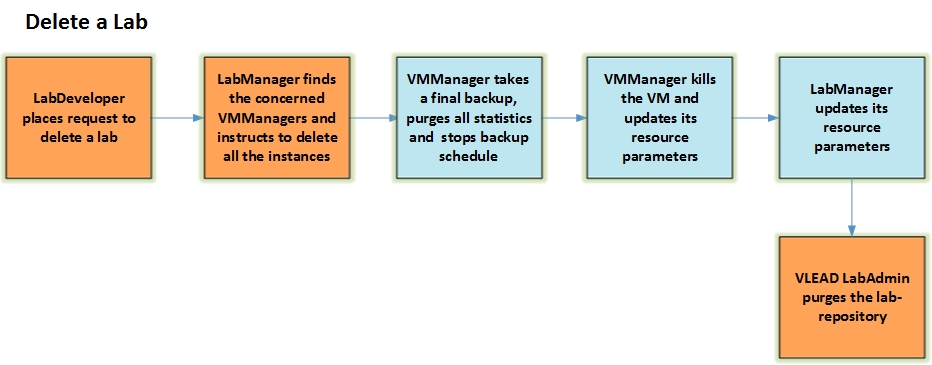
\includegraphics[width=10em]{./Delete-a-lab.jpg}

\item Fetch Lab-Statistics\\
\label{sec-3.5.1.6}

       \hyperref[sec-3.5.1.6]{ ./Fetch-lab-statistics.jpg }
\end{itemize} % ends low level
\subsubsection{Lab Administrator Workflows}
\label{sec-3.5.2}

\begin{itemize}

\item Create a Lab Repository\\
\label{sec-3.5.2.1}


\item Delete a Lab Repository\\
\label{sec-3.5.2.2}


\item Update Resource Information\\
\label{sec-3.5.2.3}

\begin{itemize}
\item Physical Machine Resources
\item Network Parameters
\item VM Manager Information
\end{itemize}

\item Update Lab Backup Schedule\\
\label{sec-3.5.2.4}


\item Take a Lab run-time snapshot\\
\label{sec-3.5.2.5}


\item Restore a Lab from its snapshot backup\\
\label{sec-3.5.2.6}


\item Deactivate a Lab\\
\label{sec-3.5.2.7}


\item Monitor VM Statistics\\
\label{sec-3.5.2.8}


\item Modify VM Run-time Parameters\\
\label{sec-3.5.2.9}


\item Purge a VM\\
\label{sec-3.5.2.10}


\item Purge VM logs\\
\label{sec-3.5.2.11}

\end{itemize} % ends low level
\subsubsection{User Workflows}
\label{sec-3.5.3}

\subsubsection{View a Lab}
\label{sec-3.5.4}

\subsubsection{Other Implicit Workflows}
\label{sec-3.5.5}

\subsubsection{Log Lab Information}
\label{sec-3.5.6}

\subsubsection{AutoPurge Lab History}
\label{sec-3.5.7}

\section{Components and Interfaces}
\label{sec-4}

\begin{itemize}
\item Following are the components that need to be designed for the proposed architecture:
\end{itemize}
\subsection{Lab Manager}
\label{sec-4.1}


\begin{description}
\item [LabOperator] Manages basic operations for the life-cycle management of lab

\begin{itemize}
\item createLab(vmmanager, lab)
\item updateLab(vmmanager, lab)
\item deleteLab(vmmanager, lab)
\item updateresources() - Adds or removes resources information (Eg. vmmanager, hosts)
\end{itemize}

\item [LabMonitor] Regularly monitors the status of labs and vms

\begin{itemize}
\item ping(vmmanager, lab)
\end{itemize}

\item [LabLogger]  Logs status and history information to the lab-info database

\begin{itemize}
\item loginfo()
\item logwarn()
\item logerror()
\item purgelogs()
\end{itemize}

\item [LabStatsCollector]

\begin{itemize}
\item collectvmstats(vmmanager)
\item collectlabstats(vmmanager, lab)
\item collectrepostats(lab)
\item updatevmstatstoDB()
\item updatelabstatstoDB()
\end{itemize}

\item [BackupManager]

\begin{itemize}
\item backup(vmmanager, lab)
\item restore(vmmanager, lab)
\item schedule(lab)
\end{itemize}

\end{description}
\subsection{VM Manager}
\label{sec-4.2}


\begin{description}
\item [VMOperator] Manages basic operations for life-cycle of a vm and a lab

\begin{itemize}
\item createvm(lab)
\item updatevm(vmid)
\item deletevm(vmid)
\item stopvm(vmid)
\item startvm(vmid)
\item updateresources(host)
\item checkoutlab(vmid, lab)
\item buildlab(vmid, lab)
\item deploylab(vmid, lab)
\item activatelab(vmid, lab)
\item testlab(vmid, lab)
\item restorelab(lab, snapshot)
\item backuplab (lab, snapshot)
\item updateinfotoDB()
\end{itemize}

\item [VMMonitor]

\begin{itemize}
\item pinglab(lab)
\item getcpuinfo(vmid)
\item getmemusage(vmid)
\item getnetworkusage(vmid)
\item getuserstats(vmid)
\item getcpuinfo(host)
\item getmemusage(host)
\item getnetworkusage(host)
\end{itemize}

\item [VMLogger]

\begin{itemize}
\item loginfo()
\item logwarn()
\item logerror()
\item purgelogs()
\end{itemize}

\item [CommandsGenerator] A component that generates the
         configuration commands based on operation specified by the
         VMOperator

\begin{itemize}
\item generateconfig(configid)
\end{itemize}

\item [CommandExecutor] A component that runs the configuration
         commands generated earlier by the CommandsGenerator

\begin{itemize}
\item applyconfig(configid)
\end{itemize}

\end{description}
    
\subsection{DeveloperPortal}
\label{sec-4.3}


\begin{itemize}
\item createdepository(lab)
\item createrepository(labdepository, lab)
\item updaterepository(labdepository, lab)
\item deleterepostitory(labdepository, l
\item deletedepository(lab)
\item sendrequest(labmanager, lab, operation) - Operation could be one of  create/update/test/release a lab or getlabstats
\item updateresources(labmanager) - Information about physical-hosts, network parameters etc
\end{itemize}
\subsection{DeploymentDashboard}
\label{sec-4.4}


\begin{itemize}
\item getlabsStatus(labmanager)
\item getlabsHistory(labInfoDb)
\end{itemize}
\subsection{LabInfoDatabase}
\label{sec-4.5}


\begin{itemize}
\item VMHistory
\item LabHistory
\item VMManagerHistory
\item LabManagerHistory
\end{itemize}
\section{Network Architecture}
\label{sec-5}

  Presented below is a network architecture diagram of the proposed
  solution:
   \href{file://../network-infrastructure.jpg }{Network}

\section{Security Architecture}
\label{sec-6}


\begin{itemize}
\item Firewall rules are configured at the router-interface for
    translating public requests to private requests.
\item Labs are accessed by users through a web-proxy that logically
    isolates the actual lab-instances from public world. In any case,
    the security of the web-proxy host is compromised. The web-proxy
    can be configured for additional security and monitored for user
    statistics. Additionally, only specific ports are enabled so that
    the labs can be accessed over web.
\item Labs are accessed by lab-developers using a gateway that isolates
    the actual lab-vms from the public world. Additionally, the
    lab-vms are proposed to be in a separate sub-network for
    additional security.
\end{itemize}
\section{Performance Model}
\label{sec-7}

\section{Reliability and Availability Model}
\label{sec-8}

\section{Backup Model}
\label{sec-9}

\begin{itemize}
\item All labs would be backup
\end{itemize}
\section{Scalablility Model}
\label{sec-10}


\end{document}
